% % % % % % % % % % % % % % % % % % % % % % % % % % % % % % % % % % % % % % % % % % % %
%                                                                                     %
% Short Sectioned Assignment LaTeX Template Version 1.0 (5/5/12)                      %
% This template has been downloaded from: http://www.LaTeXTemplates.com               %
%                                                                                     %
% Original author:  Frits Wenneker (http://www.howtotex.com)                          %
%                                                                                     %
% Modified by: Fco Javier Sueza Rodríguez (fcosueza@disroot.org)                      %
%                                                                                     %
% Changes:                                                                            %
%	    - Custom Chapters, Sections and Subsections (titlesec package)                %
%           - Document type scrbook (oneside)                                         %
%           - Use babel-lang-spanish package and marvosym                             %
%           - Use hyperref, enumitem, tcolorbox and glossaries packages               %
%           - Use Time New Roman (mathptmx), Helvetic and Courier fonts               %
%                                                                                     %
% License: CC BY-NC-SA 3.0 (http://creativecommons.org/licenses/by-nc-sa/3.0/)        %
%                                                                                     %
% % % % % % % % % % % % % % % % % % % % % % % % % % % % % % % % % % % % % % % % % % % %

%-----------------------------------------------%
%	              Packages                  %
%-----------------------------------------------%

\documentclass[paper=a4, fontsize=11pt, oneside]{scrbook}

% ---- Text Input/Output ----- %

\usepackage[T1]{fontenc}
\usepackage[utf8]{inputenc}
\usepackage{mathptmx}
\usepackage[scaled=.92]{helvet}
\usepackage{courier}
\usepackage[indent=12pt]{parskip}

\usepackage{geometry}
\geometry{verbose,tmargin=3cm,bmargin=3cm,lmargin=2.6cm,rmargin=2.6cm}

% ---- Language ----- %

\usepackage[spanish]{babel}
\usepackage{marvosym}

% ---- Another packages ---- %

\usepackage{amsmath,amsfonts,amsthm}
\usepackage{graphics,graphicx}
\usepackage{titlesec}
\usepackage{fancyhdr}
\usepackage{tcolorbox}
\usepackage{hyperref}
\usepackage{enumitem}
\usepackage[automake]{glossaries}

%--------------------------------------------------------------------%
%                      Customizing Document                          %
%--------------------------------------------------------------------%


% ----------- Custom Chapters, Sections and Subsections -------------- %

\titleformat{\chapter}[display]
			{\bfseries\Huge}
			{Tema \ \thechapter} {0.5ex}
			{\vspace{1ex}\centering}

\titleformat{\section}[hang]
			{\bfseries\Large}
			{\thesection}{0.5em}{}

\titleformat{\subsection}[hang]
			{\bfseries\large}
			{\thesubsection}{0.5em}{}

\titleformat{\subsubsection}[hang]
			{\bfseries\large}
			{\thesubsubsection}{0.5em}{}

\hypersetup{
    colorlinks=true,
    linkcolor=black,
    urlcolor=magenta
}

% ------------------- Custom heaaders and footers ------------------- %

\pagestyle{fancyplain}

\fancyhead[]{}
\fancyfoot[L]{}
\fancyfoot[C]{}
\fancyfoot[R]{\thepage}

\renewcommand{\headrulewidth}{0pt} % Remove header underlines
\renewcommand{\footrulewidth}{0pt} % Remove footer underlines

\setlength{\headheight}{13.6pt} % Customize the height of the header

% --------- Numbering equations, figures and tables ----------------- %

\numberwithin{equation}{section} % Number equations within sections
\numberwithin{figure}{section} % Number figures within sections
\numberwithin{table}{section} % Number tables within sections

% ------------------------ New Commands ----------------------------- %

\newcommand{\horrule}[1]{\rule{\linewidth}{#1}} % Create horizontal rule command


%----------------------------------------------------------------------------------------
%	TÍTULO Y DATOS DEL ALUMNO
%----------------------------------------------------------------------------------------

\title{
\vspace{10ex}
\normalfont \normalsize
\Huge \textbf{Tarea 1: Conociendo Mi Equipo}
}
\author{Francisco Javier Sueza Rodríguez}
\date{\normalsize\today}

%----------------------------------------------------------------------------------------
%                                     DOCUMENTO
%----------------------------------------------------------------------------------------
\begin{document}

\maketitle

\thispagestyle{empty}

\vspace{75ex}

\begin{center}
    \begin{tabular}{l l}
        \textbf{Centro}: & IES Aguadulce \\
        \textbf{Ciclo Formativo}: & Desarrollo Aplicaciones Web (Distancia)\\
        \textbf{Asignatura}: & Sistemas Informáticos\\
        \textbf{Tema}: & Tema 1 -  Hardware de un Sistema Informático\\
    \end{tabular}
\end{center}

\newpage

\tableofcontents

\vspace{15ex}

\hrule

\vspace{10ex}

\listoffigures

\newpage

\section{Caso Práctico}
José Manuel quiere montar un ordenador para su hermana pequeña, principalmente para jugar a videojuegos modernos y poder realizar tareas que requieran cierta potencia de computación, como la elaboración de contenidos audiovisuales; pero José Manuel no tiene muchos conocimientos de hardware. Ada le ha sugerido que pida ayuda a Juan y a María para que le enseñen los conceptos básicos sobre hardware.

José Manuel hace lo que Ada le sugiere, y Juan y María deciden empezar por enseñar a José Manuel a analizar los componentes de su propio equipo, para que vaya familiarizándose con los mismos.

\section{Actividades}
En esta sección se incluyen todas las actividades, divididas en subsecciones con su correspondiente descripción y su solución.

\subsection{Actividad 1: Resumen de Hardware}
Descarga y ejecuta el programa gratuito HWiNFO en tu equipo (se recomienda la versión "portable" ya que no requiere instalación). Una vez dentro, incluye en el documento de la tarea lo siguiente:

\begin{itemize}
    \item Una captura de la ventana "resumen del sistema" (consultar el ejemplo de solución en caso de duda), donde se resumen las principales características del equipo. En esta captura señala de manera clara (un recuadro, un subrayado, etc.) los siguientes datos:

    \begin{itemize}
        \item El modelo de la placa base y su chipset.
        \item El modelo de la CPU.
        \item El modelo de la GPU.
        \item Tipo, cantidad y velocidad de la memoria RAM.
        \item Las opciones de virtualización de la CPU. Esto aparece en el apartado "características", con el nombre "VMX" o "VT-x" si tu procesador Intel, o "AMD-V" o "SVM" si tu procesador es AMD. En caso de que dicha opción aparezca en rojo en lugar de verde, debes entrar en la BIOS/UEFI de tu equipo y habilitar las opciones de virtualización de tu procesador (esta opción puede tener distintos nombres según la placa base). Esto es necesario de cara a futuras tareas.
    \end{itemize}

    \item A continuación, copia y pega el texto generado en el "resumen para portapapeles" (Reporte > Resumen para portapapeles).
\end{itemize}

Si usas un sistema operativo GNU/Linux puedes utilizar otros programas como "hardinfo" o "CPU-X". En el caso de equipos Mac puedes usar "menú Apple > Acerca de este Mac". En estos casos intenta recopilar la información básica de: CPU, placa base, chipset, memoria RAM, gráficos, unidades de almacenamiento, sonido, red y sistema operativo (una línea por cada componente).

\subsubsection{Solución}
Se ha usado el software \textbf{HWiNFO} para obtener la información sobre el hardware. El modelo del ordenador es un portátil \textbf{HP-15s-eq0003ns}. En la siguiente figura, se muestra la captura de pantalla pedida con la información sobre el hardware.

\begin{figure}[ht]
    \centering
    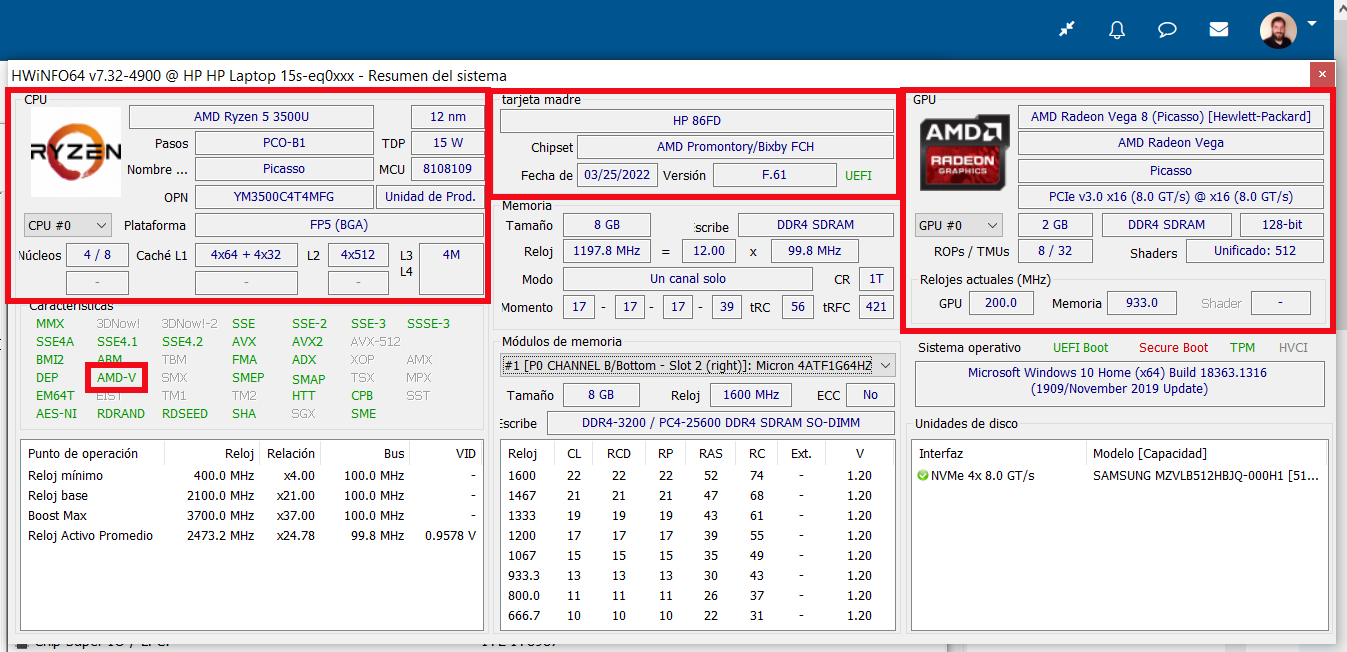
\includegraphics[scale=0.54]{info-sistema.png}
    \caption{Información hardware de HWiNFO}
\end{figure}

A continuación vemos el informe generado por HWiNfo usando la opción ``\textbf{Resumen para portapapeles}''.

\begin{figure}[ht]
    \begin{tcolorbox}[sharp corners, colback=yellow!30, colframe=white!20]
\begin{center}
    \begin{tabular}{p{6em} p{31em}}
        Computer:   &  HP HP Laptop 15s-eq0xxx \\
        CPU:        &  AMD Ryzen 5 3500U (Picasso, PCO-B1) 2100 MHz (21.00x100.0) @ 1834 MHz (18.38x99.8) \\
        Motherboard:&  HP 86FD  \\
        BIOS:       &  F.61, 03/25/2022 \\
        Chipset:    &  AMD Promontory/Bixby FCH \\
        Memory:     &  8192 MBytes @ 1197 MHz, 17-17-17-39 - 8192 MB PC25600 DDR4 SDRAM - Micro 4ATF1G64HZ-3G2E1 \\
        Graphics:   &  AMD Radeon Vega 8 (Picasso) [Hewlett-Packard] AMD Radeon Vega, 2048 MB DDR4 SDRAM \\
        Drive:      &  SAMSUNG MZVLB512HBJQ-000H1, 500.1 GB, NVMe \\
        Sound:      &  ATI/AMD Display HD Audio Controller \\
        Sound:      &  AMD Zen - Audio Processor - HD Audio Controller \\
        Network:    &  RealTek Semiconductor, Device ID: C821 \\
        OS:         &  Microsoft Windows 10 Home (x64) Build 18363.1316 (1909/November 2019 Update) \\
    \end{tabular}
\end{center}
    \end{tcolorbox}
    \caption{Reporte para portapapeles de HWiNFO}
\end{figure}

\subsection{Actvidad 2: Características de la CPU y la GPU}
Utilizando como base la información que has obtenido en la actividad 1, busca la siguiente información detallada, bien en las páginas web oficiales de los fabricantes o utilizando software gratuito como HWiNFO, CPU-Z, GPU-Z, etc.:

\begin{itemize}
    \item De la CPU:
    \begin{itemize}
        \item Fabricante.
        \item Modelo.
        \item Fecha de salida al mercado.
        \item Número de núcleos y subprocesos (cores/threads)
        \item Velocidad base en GHz, si la tiene
        \item Velocidad turbo o boost en GHz, si la tiene.
        \item Tamaño de caché.
        \item Tamaño del proceso de fabricación (litografía) en "nm".
        \item  TDP en vatios.
    \end{itemize}
    \item Del adaptador gráfico:
    \begin{itemize}
        \item Indica si es una iGPU (GPU integrada en el procesador o chipset) o una GPU dedicada (tarjeta gráfica no integrada). Si tu equipo tiene ambos, elige la GPU dedicada.
        \item Fabricante del chip gráfico (Nvidia, AMD, Intel).
        \item Chip gráfico de la tarjeta (mirar ejemplo de solución).
        \item Modelo exacto.
        \item Cantidad y tipo de memoria VRAM (RAM de vídeo).
    \end{itemize}
\end{itemize}

\subsubsection{Solución}

En primer lugar se va a mostrar la información relativa al procesador, en este caso un \textbf{Ryzen 5 3500U}, en la siguiente tabla. La información ha sido obtenida de la página oficial de AMD. \cite{amd01}:

\begin{figure}[ht]
    \centering

    \setlength{\tabcolsep}{10pt}
    \renewcommand{\arraystretch}{1.5}

    \begin{tabular}{| p{10em} | p{15em} |}
        \hline
        \textbf{Fabricante}       &  AMD \\ \hline
        \textbf{Modelo}           &  AMD Ryzen 5 3500U ("Picasso") \\ \hline
        \textbf{Nucleos}          &  4 \\ \hline
        \textbf{Threads}          & 8 \\ \hline
        \textbf{Velocidad Base}   &  2.1GHz \\  \hline
        \textbf{Velocidad Turbo}  &  3.7GHz  \\ \hline
        \textbf{Cache L1}  		  & 384KB  \\ \hline
        \textbf{Cache L2} 	      & 2MB  \\ \hline
        \textbf{Cache L3}  	      & 4MB  \\ \hline
        \textbf{Litografía}	      & 12nm   \\  \hline
        \textbf{TDP Defecto}      & 15W \\ \hline
        \textbf{TDP Configurable} & 12-35W \\
        \hline
    \end{tabular}
    \caption{Información de la CPU}
\end{figure}

A continuación se muestra la información referida a la GPU, una gráfica integrada \textbf{AMD Radeon Vega 8}. La información ha sido obtenida con la aplicación \textbf{HWiNfo}.

\begin{figure}[ht]

    \vspace{3ex}
    \centering

    \setlength{\tabcolsep}{10pt}
    \renewcommand{\arraystretch}{1.5}

    \begin{tabular}{| p{10em} | p{20em} |}
        \hline
        \textbf{Tipo de GPU}  &  GPU integrado \\ \hline
        \textbf{Fabricante}   &  AMD \\ \hline
        \textbf{Chip Gráfico} &  AMD Radeon Vega\\ \hline
        \textbf{Modelo}       &  AMD Radeon Vega 8 (Picasso) \\ \hline
        \textbf{VRAM}         &  2 GB DDR4 SDRAM (Memoria Compartida) \\
        \hline
    \end{tabular}
    \caption{Información de la GPU}
\end{figure}

\subsection{Actividad 3: Características de la Placa Base}
Para esta actividad vas a usar tu propia placa base y su manual como referencia. Si no lo tienes en papel, es fácil descargarse el manual de tu placa base conociendo el modelo exacto (lo hemos conocido en la ``Actividad 1''), buscándolo en Internet y accediendo al apartado de ``soporte'' o ``descargas'' de la web oficial del producto. En dicho manual encontrarás imágenes en las que se detalla dónde se sitúan todos los componentes de la placa base.

Si tu equipo es portátil o es un equipo pre-ensamblado es posible que acceder a un manual similar sea difícil o imposible. En ese caso, utiliza la siguiente placa base para la actividad: ``MSI MAG Z590 Tomahawk WIFI''.

\begin{itemize}
    \item \textbf{Primero:} Incluye una captura de la portada del manual o la página del mismo en la que se muestre el modelo de la placa base, para comprobar que es el manual correcto. Recuerda que en la captura se debe mostrar tu usuario de la plataforma (sin ser un collage)

    \item \textbf{Segundo:} Sobre una fotografía superior de la placa base (se puede descargar en el apartado de ``galería'' de su página web, pero debe ser una fotografía y no el diagrama que se incluye en el manual), localiza y señala los siguientes componentes usando los números que se indican:
    \begin{itemize}
        \item Conectores de alimentación:
        \begin{itemize}
            \item (1) ATX 20+4 pines.
            \item (2) ATX 12V para alimentación de la CPU .
        \end{itemize}
        \item (3) Zócalo de la CPU (indica el nombre exacto del zócalo).
        \item (4) Conector de ventilador/refrigeración de la CPU .
        \item (5) Ranuras de memoria RAM (indica el tipo de RAM: DDR3, DDR4...).
        \item (6) Chipset (indica el nombre exacto del chipset).
        \item Almacenamiento
        \begin{itemize}
            \item (7) Puertos SATA.
            \item (8) Ranuras M.2 (si las tiene).
        \end{itemize}
        \item (9) Ranuras de expansión (indicando el tipo: PCI, PCIe x1, PCIe x16, etc.).
        \item (10) Batería de la CMOS (pila de botón CR2032).
        \item (11) Conectores internos del panel frontal (botones de encendido, reset y leds frontales).
        \item (12) Cabeceras internas para USB 2.x o 3.x frontales.
        \item (13) Cabecera interna para el audio frontal.
        \item Tras la fotografía, incluye una tabla con tantas filas como números y tres columnas en la que indiques: número, nombre del componente, función del mismo.
    \end{itemize}

    \item \textbf{Tercero:} Sobre una fotografía del panel trasero de la placa base, señala con letras (A, B, C...) cada uno de los puertos/elementos traseros (se pueden agrupar los que sean exactamente iguales y con las mismas características).
    \begin{itemize}
        \item
        Tras la fotografía incluye una tabla con tantas filas como letras y tres columnas en la que indiques: letra, nombre del elemento, función del mismo.
    \end{itemize}
\end{itemize}

\subsubsection{Solución}
Para esta actividad se va a usar la placa base ``\textbf{MSI MAG Z590 Tomahawk WIFI}'', ya que aunque sabemos que el modelo de la placa base del portátil es una \textbf{HP 86FD}, es muy complicado encontrar el manual, y más aún acceder a ella para poder fotografiarla, por lo que se empleará la placa base que proporciona el enunciado de la actividad como modelo.

\begin{enumerate}
    \item \textbf{Manual}: en primer lugar vamos a mostrar una imagen del manual de la placa base donde aparezca el modelo, para asegurarnos de que es el correcto. El manual se ha descargado desde la página de soporte de MSI. \cite{msi01}

    \begin{figure}[ht]
        \centering
        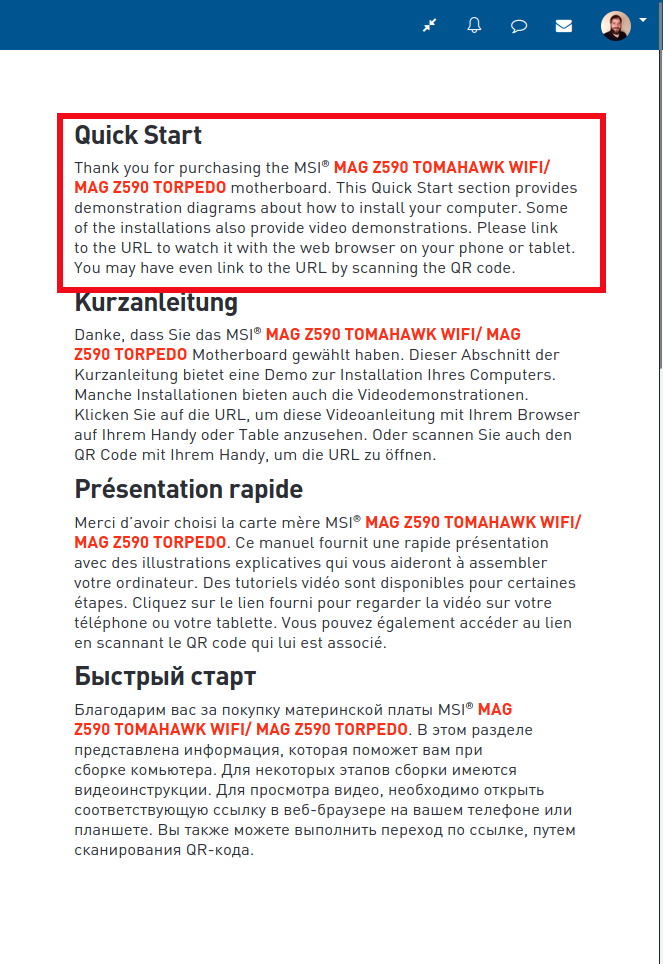
\includegraphics[scale=0.40]{manual-placa.png}
        \caption{Manual placa base MSI MAG Z590 Tomahawk}
    \end{figure}

    \item \textbf{Componentes Placa Base}: a continuación se muestra la imagen superior de la placa base y se indican cada uno de los componentes que se solicitan. La imagen ha sido descargada de la sección ``Galería'' de la página correspondiente a la placa base en la página oficial de MSI. \cite{msi02}

    \begin{figure}[ht]
        \centering
        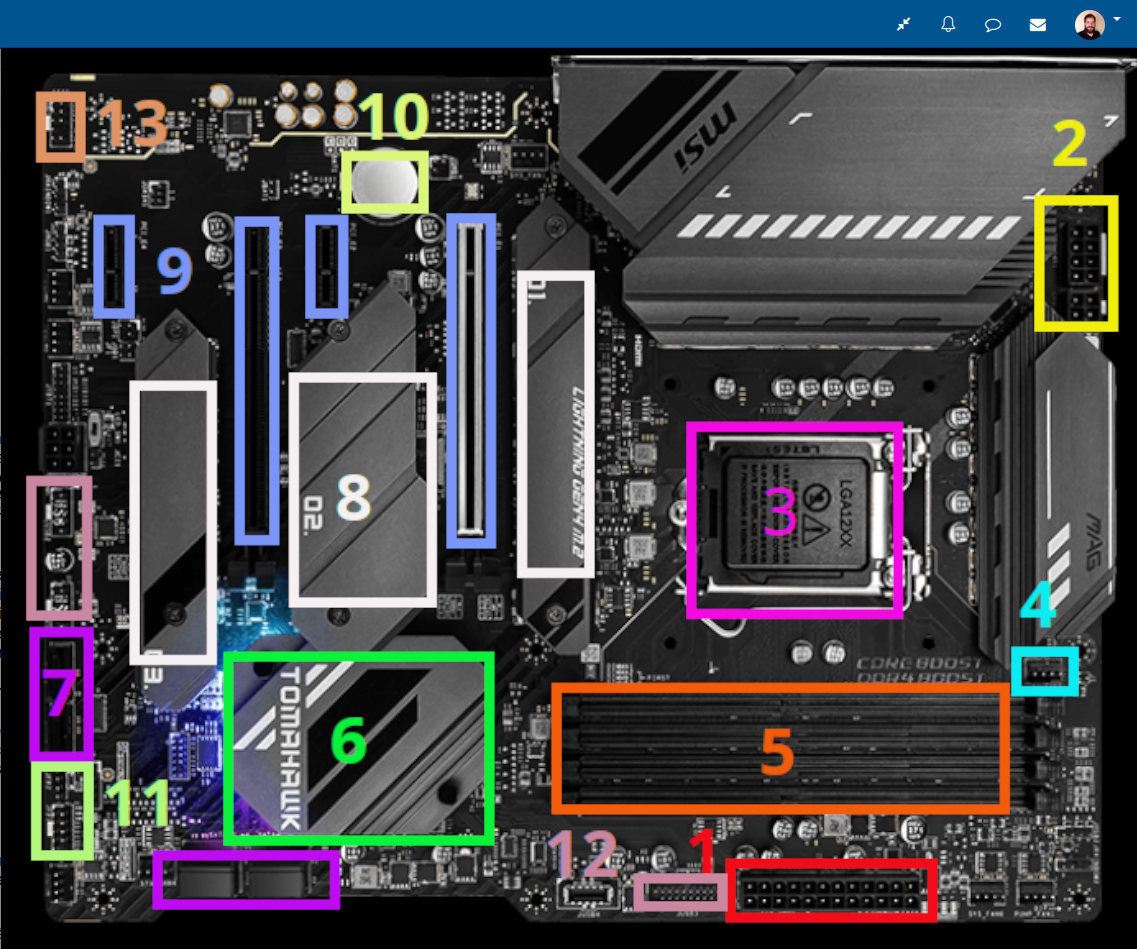
\includegraphics[scale=0.32]{placa-base-tomahawk.png}
        \caption{Vista superior de placa base y conectores}
    \end{figure}

    A continuación se muestra la tabla con todos los componentes señalados en la figura anterior, incluyendo su modelo y función.

    \begin{figure}[ht]
        \centering
        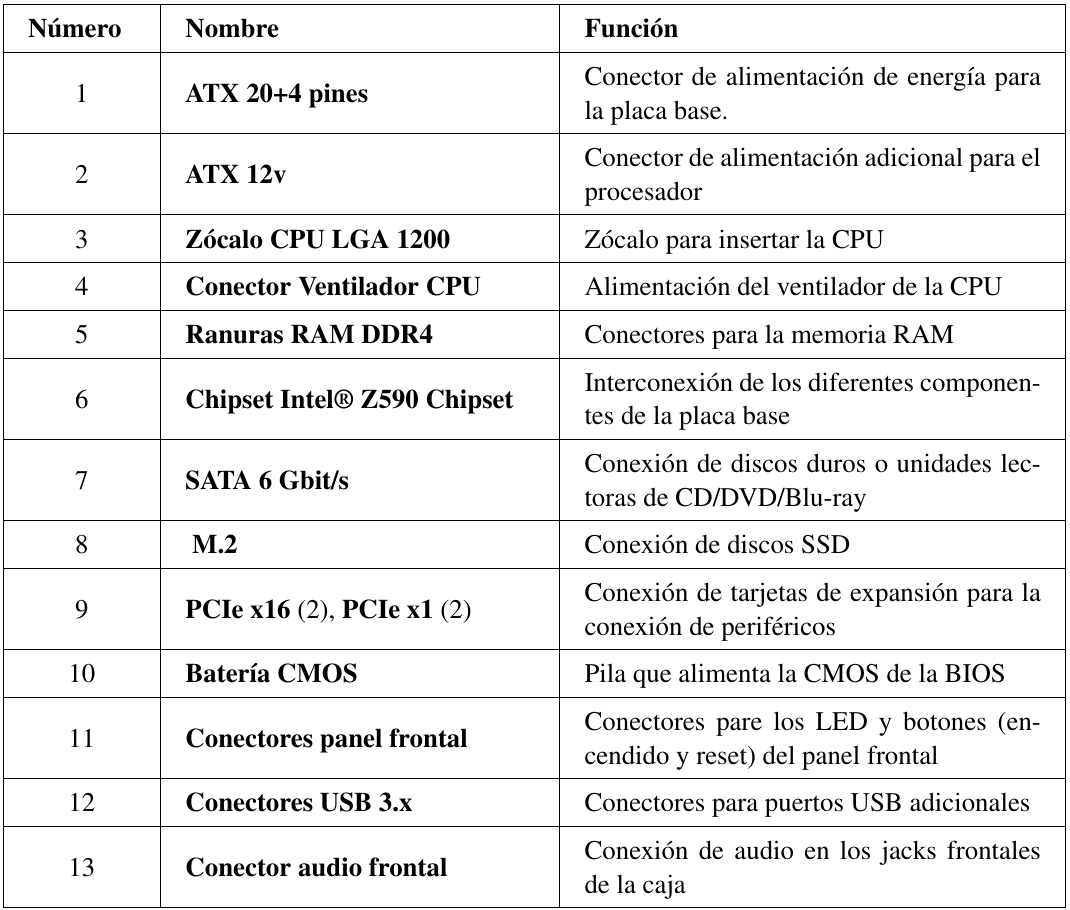
\includegraphics[scale=0.32]{tabla-specs.png}
        \caption{Tabla con las especificaciones de los conectores}
    \end{figure}

    \item \textbf{Panel trasero de la Placa}: por último, mostramos el panel trasero de la placa base, al cual podremos acceder, una vez montada, desde la parte trasera de la caja. Se indican los diferentes tipos de conectores que tiene agrupándolos según su funcionalidad.

    \vspace{4em}

    \begin{figure}[ht]
        \centering
        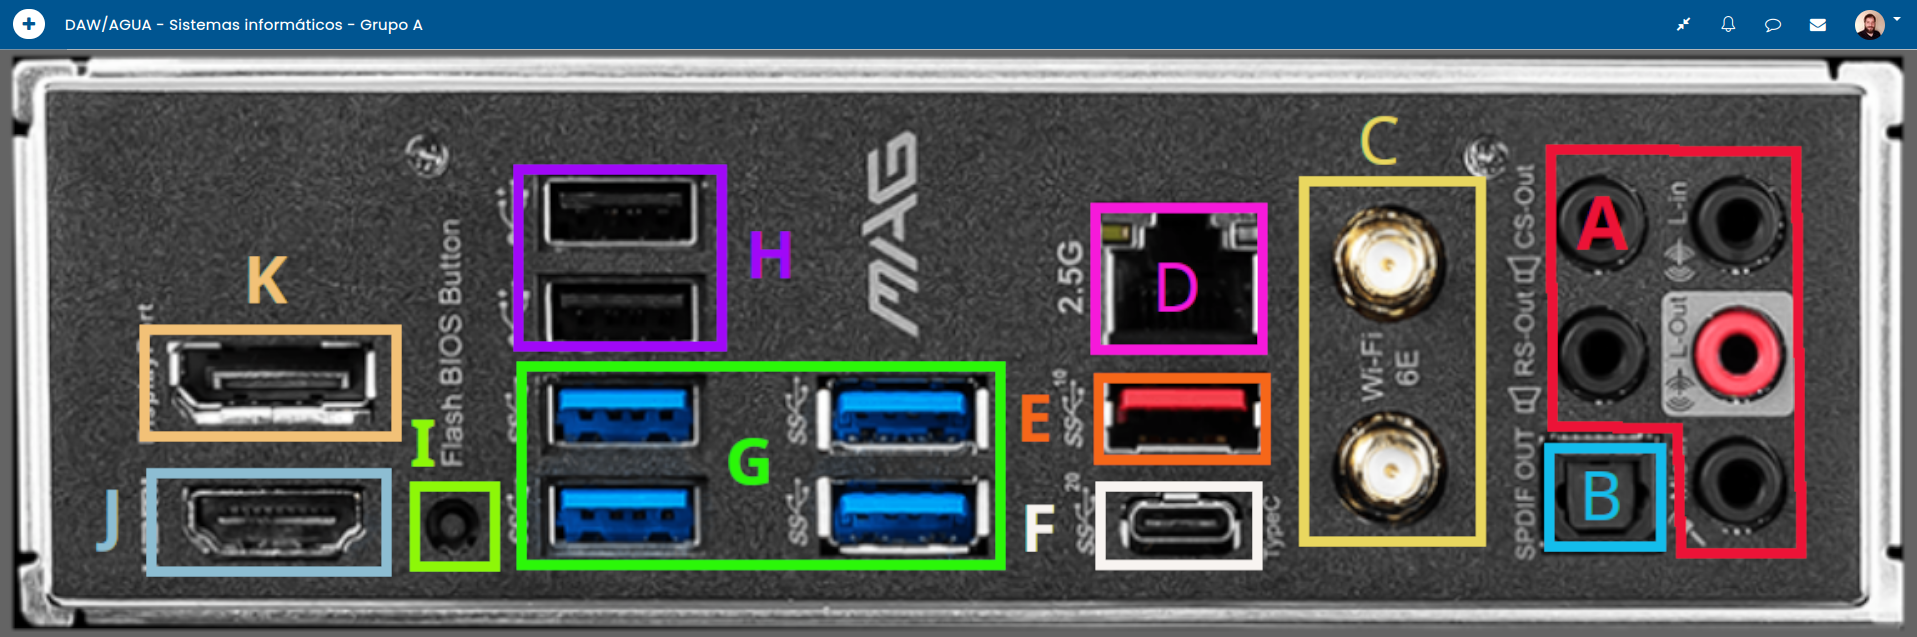
\includegraphics[scale=0.22]{panel-trasero-placa.png}
        \caption{Parte trasera de la placa base}
    \end{figure}

    A continuación, se muestra la tabla explicando como se llama cada conexión y cual es su utilidad.

    \begin{figure}[ht]

        \vspace{3ex}
        \centering

        \setlength{\tabcolsep}{10pt}
        \renewcommand{\arraystretch}{1.4}

        \begin{tabular}{| m{4em} | m{13em} | m{16em} |}
            \hline
            \textbf{Letra}  & \textbf{Nombre} & \textbf{Función} \\ \hline
            \centering A &  Puertos de Audio & Conexiones de entrada/salida para dispositivos de audio \\ \hline
            \centering B &  Salida S/PDIF  & Conexión de salida para audio digital \\ \hline
            \centering C &  Conectores de antena Wi-Fi & Sirven para conectar una antena Wi-Fi \\ \hline
            \centering D &  Puerto Ethernet & Puerto de entrada/salida ethernet para conectar el ordenador a una red local o a internet \\ \hline
            \centering E &  USB 3.2 Gen 2 & Conexión de dispositivos mediante USB, velocidad de hasta 10Gb/s \\ \hline
            \centering F &  USB 3.2 Gen 2x2 & Conexión de dispositivos mediante USB, velocidad de hasta 20Gb/s \\ \hline
            \centering G &  USB 3.2 Gen 1 & Conexión de dispositivos mediante USB, velocidad de hasta 5Gb/s \\ \hline
            \centering H &  USB 2.0 Tipo A & Conexión de dispositivos mediante USB y conector de tipo A \\ \hline
            \centering I &  Botón Flash BIOS & Se utiliza para actualizar la BIOS \\ \hline
            \centering J &  HDMI & Salida HDMI para conectar un monitor \\ \hline
            \centering K &  Display Port & Salida para conectar un monitor \\
            \hline
        \end{tabular}
        \caption{Tabla de conectores de la placa base}
    \end{figure}
\end{enumerate}

\subsection{Actividad 4: Preguntas Sobre la Placa Base}
Utilizando la misma placa base que usaste para la actividad 3, contesta a las siguientes preguntas. Cada contestación debe ser escrita, e ir acompañada de una imagen que muestre el apartado del manual del que se ha obtenido la información (recuerda que las capturas deben mostrar tu usuario de la plataforma, sin ser un collage):

\begin{enumerate}
    \item ¿Qué procesadores soporta?
    \item ¿Cuál es su factor de forma y qué dimensiones exactas tiene?
    \item ¿Qué puertos/ranuras dispone para dispositivos de almacenamiento?
    \item Puertos USB: Indica cuántos tiene, si son traseros o disponibles mediante cabeceras internas, y di de qué versión son (USB 2.0, USB 3.0, USB 3.2 gen2, etc.).
    \item ¿Cuántas ranuras de memoria tiene y qué tipo de memoria acepta? Indica tipo (DDR3, DDR4, DDR5...) y máxima memoria soportada.
    \item ¿Incorpora firmware de tipo BIOS ``clásica'' o UEFI? ¿Qué es UEFI y en qué se diferencia de las BIOS clásicas?
    \item Busca el diagrama de bloques (``block diagram'') en el manual de la placa base (si tu manual no lo incorpora, búscalo para la placa base ``MSI MAG Z590 Tomahawk WIFI'' en su manual en inglés, ya que la versión multi-idioma del manual no lo incluye). Hazle una captura de pantalla y coméntalo brevemente.
    \item Busca en la web de la placa base, en el apartado de ``soporte'' o ``compatibilidad de CPU'', la lista completa de CPU compatibles con la placa base. ¿Cuál es la CPU más potente soportada por la placa base? Haz una captura de dicha página en la que se vea la que creas que es la CPU con mayor capacidad de computación soportada por la placa base. No es necesario que se vea la lista completa. (Si tienes dudas acerca del rendimiento de los procesadores puedes usar como referencia la web de pruebas de rendimiento \url{https://www.cpubenchmark.net/}).
\end{enumerate}

\subsubsection{Solución}
En este apartado se responderán a todas las preguntas, la información se ha extraído del manual de usuario de la placa base, descargado de la página oficial de MSI, en su versión en inglés. \cite{msi03}
\begin{enumerate}
    \item \textbf{¿Qué procesadores soporta?}

    Esta placa base tiene un \textbf{socket LGA 1200} por lo que soporta procesadores \textbf{Intel® Core™} de \textbf{10ª} y \textbf{11ª generación}, así como procesadores \textbf{Pentium® Gold} y \textbf{Celeron®}.

    \begin{figure}[ht]
        \centering
        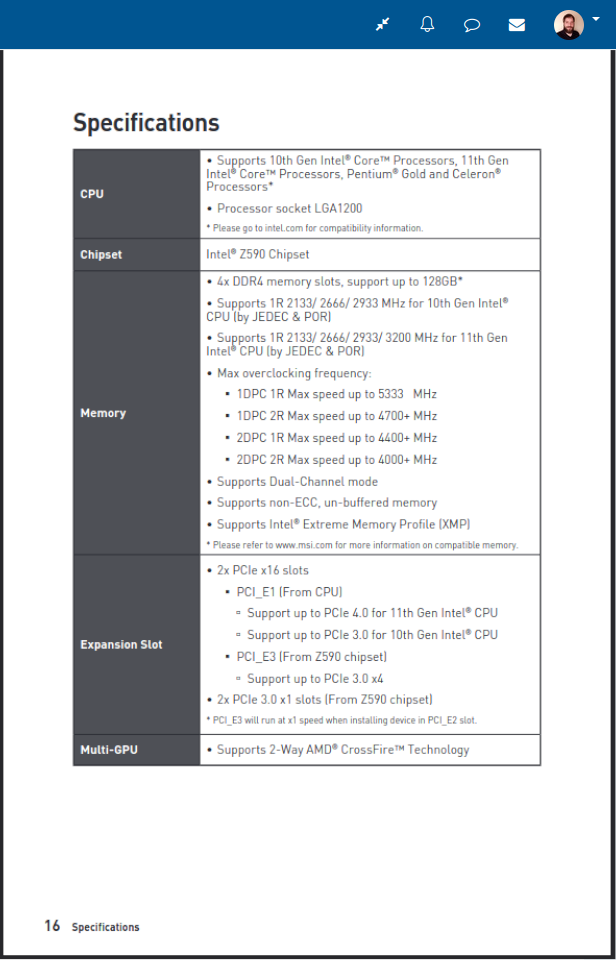
\includegraphics[scale=0.30]{manual-procesador.png}
        \caption{Página 16 del manual de usuario}
    \end{figure}

    \item \textbf{¿Cuál es su factor de forma y qué dimensiones exactas tiene?}

    La placa base tiene un factor de forma \textbf{ATX} y sus medidas exactas son de \textbf{30.5 cm} x \textbf{24.4 cm}

    \begin{figure}[ht]
        \centering
        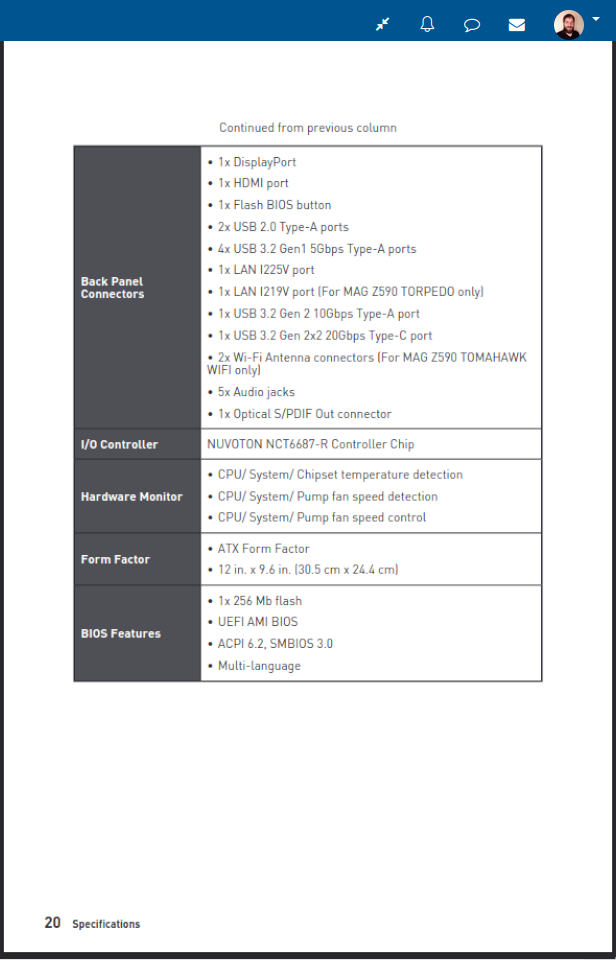
\includegraphics[scale=0.30]{manual-forma.png}
        \caption{Página 20 del manual de usuario}
    \end{figure}

    \item \textbf{¿Qué puertos/ranuras dispone para dispositivos de almacenamiento?}

    La placa base tiene \textbf{6 puertos SATA 6Gb/s} y \textbf{3 ranuras M.2}. Las ranuras M.2 están controladas 1 por la CPU y las otras 2 por el chipset Z590, mientras que los puertos SATA están todos controlados por el chipset.

    \begin{figure}[ht]
        \centering
        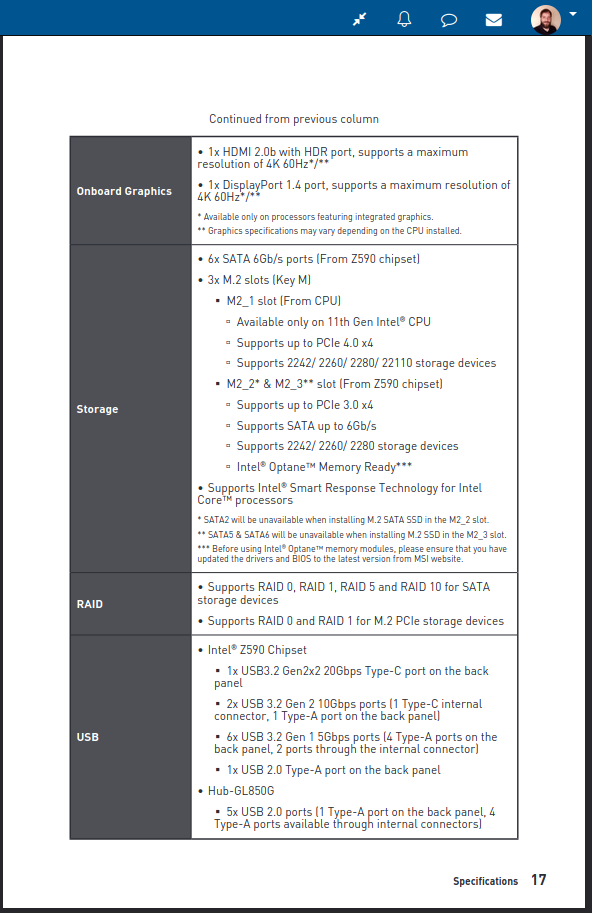
\includegraphics[scale=0.30]{manual-almacenamiento.png}
        \caption{Página 17 del manual de usuario}
    \end{figure}

    \item \textbf{Puertos USB: Indica cuántos tiene, si son traseros o disponibles mediante cabeceras internas, y di de qué versión son (USB 2.0, USB 3.0, USB 3.2 gen2, etc.).}

    La placa base dispone de los siguientes puertos USB:
    \begin{itemize}
        \item 1x \textbf{USB 3.2 Gen 2x2 Tipo C} (panel trasero)
        \item 2x \textbf{USB 3.2 Gen 2}:
        \begin{itemize}
            \item 1x \textbf{Tipo C} (conector interno)
            \item 1x \textbf{Tipo A} (panel trasero)
        \end{itemize}
        \item 6x \textbf{USB 3.2 Gen 1}:
        \begin{itemize}
            \item 4x \textbf{Tipo A} (panel trasero)
            \item 2x puertos (conector interno)
        \end{itemize}

        \item 6x \textbf{USB 2.0}:
        \begin{itemize}
            \item 2x \textbf{Tipo A} (panel trasero)
            \item 4x \textbf{Tipo A} (conector interno)
        \end{itemize}
    \end{itemize}

    Esta información se ha obtenido de la página 17 del manual. En la Figura 2.12 puede verse la captura relativa a esta página, aún así se incluirá en este a apartado (de nuevo) en caso de que sea necesaria.

    \begin{figure}[ht]
        \centering
        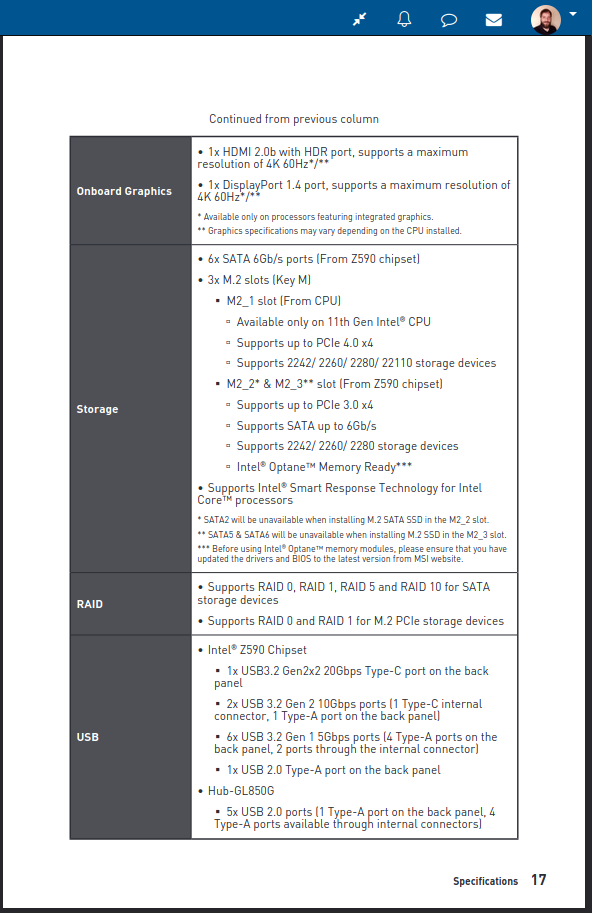
\includegraphics[scale=0.30]{manual-almacenamiento.png}
        \caption{Página 17 del manual de usuario}
    \end{figure}

    \item \textbf{¿Cuántas ranuras de memoria tiene y qué tipo de memoria acepta? Indica tipo (DDR3, DDR4, DDR5...) y máxima memoria soportada.}

    Esta placa base tiene \textbf{4 ranuras} de memoria de tipo \textbf{DDR4} y suporta hasta \textbf{128 GB} de memoria. Soporta el \textbf{modo Dual-Channel}, memoria \textbf{non-ECC} y \textbf{Intel® Extreme Memory Profile}. Respecto a las frecuencias, depende el procesador que instalemos soporta unas u otras:
    \begin{itemize}
        \item \textbf{Procesadores Intel® de 10ª Generación}: 2133/2666/2933 MHz
        \item \textbf{Procesadores Intel® de 11ª Generación}: 2133/2666/2933/3200 MHz
    \end{itemize}

    Esta información se ha obtenido de la página 16 del manual. En la Figura 2.10 puede verse la captura relativa a esta página, aún así se incluirá en este a apartado (de nuevo) en caso de que sea necesaria.

    \begin{figure}[ht]
        \centering
        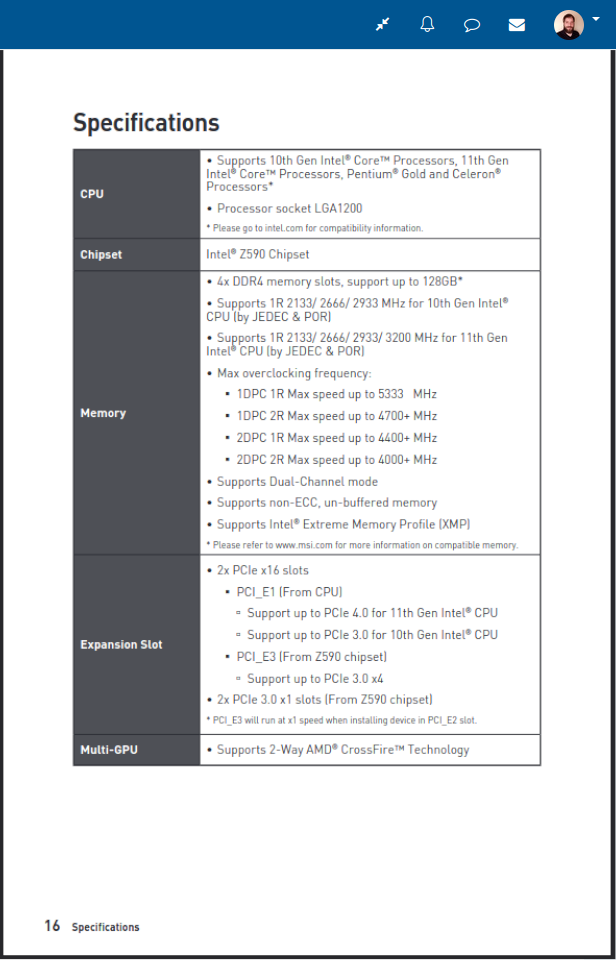
\includegraphics[scale=0.30]{manual-procesador.png}
        \caption{Página 16 del manual de usuario}
    \end{figure}

    \item \textbf{¿Incorpora firmware de tipo BIOS ``clásica'' o UEFI? ¿Qué es UEFI y en qué se diferencia de las BIOS clásicas?}

    Esta placa base incorpora una \textbf{BIOS UEFI} (Unified Extensible Firmware Interface), como la mayoría de los ordenadores modernos.

     Según el propio manual de la placa base, algunas de las \textbf{ventajas} de estos tipos de BIOS respecto a las clásicas son las siguientes:
    \begin{itemize}
        \item \textbf{Inicialización más rápida}: las BIOS UEFI pueden inicializar el sistema operativo directamente salvando el proceso de auto-testeo de la BIOS. Además elimina el tiempo para cambiar el modo CMS (Compatibility Support Mode) durante el POST de la BIOS.

        \item Soporte para \textbf{particiones} de disco duro \textbf{superiores a 2 TB}.
        \item Soporte para \textbf{más de 4 particiones primarias} con particiones de tablas GUID (GPT).
        \item Soporte para un \textbf{número ilimitado de particiones}.
        \item Soporta todas las capacidades de los nuevos dispositivos. Algunos pueden no tener retrocompatibilidad.
        \item Soporta \textbf{inicialización segura}: las BIOS UEFI pueden comprobar la validez del sistema operativo para asegurarse de que no hay malware.
    \end{itemize}

    Aunque las BIOS UEFI tienen muchísimas ventajas, también tienen algunas \textbf{desventajas} que las diferencia de las BIOS clásicas, las principales son la siguientes dos:

    \begin{itemize}
        \item Estás placas base no tienen soporte para Microsoft Windows de 32-bits, solo soportan su versión de 64-bits.
        \item Pueden general problemas con tarjetas gráficas antiguas, en cuyo caso se nos mostrará un mensaje indicándonos que no hay soporte dicha tarjeta gráfica.

        En este último supuesto, lo recomendable es cambiar a una tarjeta gráfica que tenga soporte para GOP/UEFI o usar la tarjeta gráfica integrada en la CPU.
    \end{itemize}

    \begin{figure}[ht]
        \centering
        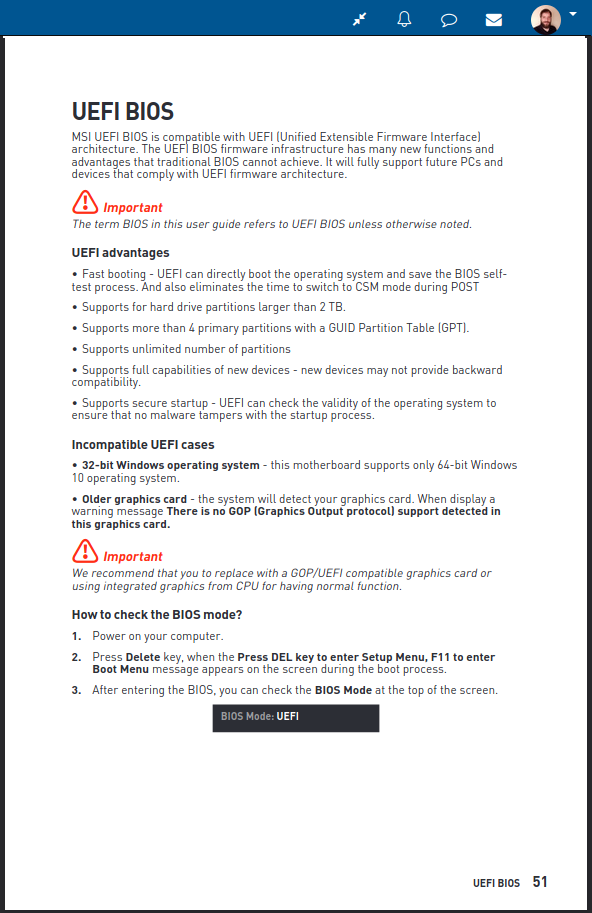
\includegraphics[scale=0.30]{manual-uefi.png}
        \caption{Página 51 del manual de usuario}
    \end{figure}

    \item  \textbf{Busca el diagrama de bloques (``block diagram'') en el manual de la placa base (si tu manual no lo incorpora, búscalo para la placa base ``MSI MAG Z590 Tomahawk WIFI'' en su manual en inglés, ya que la versión multi-idioma del manual no lo incluye). Hazle una captura de pantalla y coméntalo brevemente.}

    En este apartado vamos a echarle un vistazo al diagrama de bloques de la placa base que estamos tratando. En la siguiente figura, podemos ver el diagrama, que se a obtenido del manual de usuario oficial. \cite{msi03}

    \begin{figure}[ht]
        \centering
        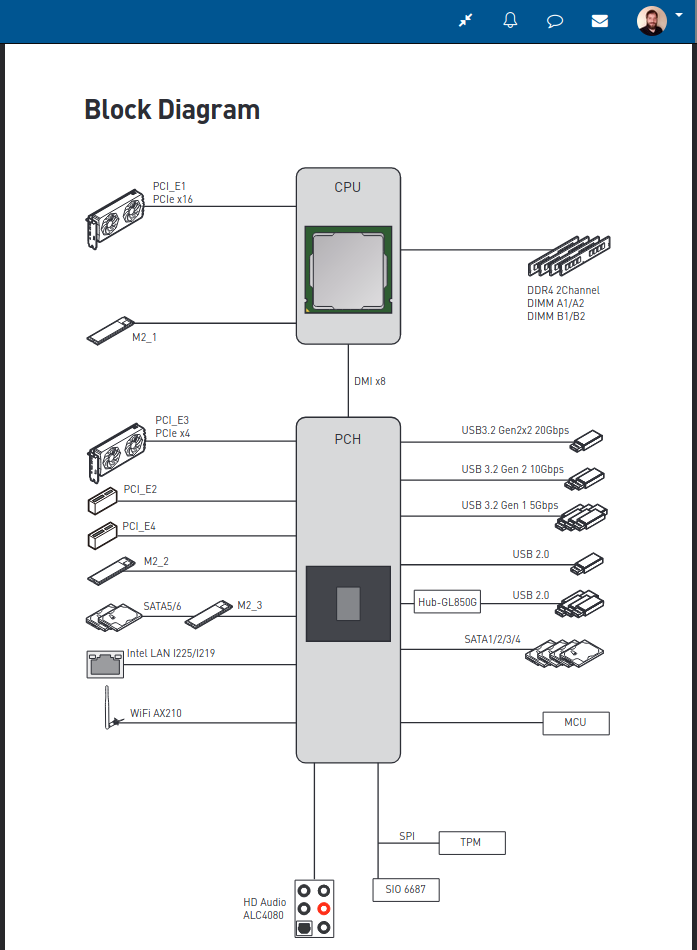
\includegraphics[scale=0.33]{diagrama-bloques.png}
        \caption{Diagrama de bloques de la placa base}
    \end{figure}

    Una de las cosas que nos puede llamar la atención al ver el diagrama de bloques, es que no vemos el \textbf{Northbridge} ni el \textbf{Souhtbridge} por ningún lado, tampoco vemos el \textbf{FSB}, sino una canal \textbf{DMI} entre el chipset y la CPU. Esto se debe a que esta es una arquitectura \textbf{PCH} (Platform Chipset Hub). Esta es una arquitectura de chipset de un solo chip introducida por Intel en 2009 como sustituta de su anterior arquitectura, Intel Hub Architecture, que si usaba dos chips (Northbridge - Southbridge).

    En esta arquitectura, algunas de las funciones del Northbrigde, como el control de la memoria RAM y alguna ranura PCIe, están integradas en la CPU, mientras que el PCH se encarga del resto de funciones, incluidas las propias del Southbridge. \cite{wiki01}

    Además, se ha sustituido el FSB por un canal DMI (Direct Media Transport), que es la tecnología propietaria de Intel, que sustituye al FSB y que llevan usando desde hace años, en un principio como enlace entre el Northbridge y el Southbridge y actualmente entre el PCH y la CPU o la RAM. \cite{wiki02}

     \item \textbf{Busca en la web de la placa base, en el apartado de ``soporte'' o ``compatibilidad de CPU'', la lista completa de CPU compatibles con la placa base. ¿Cuál es la CPU más potente soportada por la placa base? Haz una captura de dicha página en la que se vea la que creas que es la CPU con mayor capacidad de computación soportada por la placa base. No es necesario que se vea la lista completa. (Si tienes dudas acerca del rendimiento de los procesadores puedes usar como referencia la web de pruebas de rendimiento \url{https://www.cpubenchmark.net/})}

     En este apartado hemos visitado la página de soporte de MSI para la placa base, en la sección de compatibilidad \cite{msi04}.

     Aunque en la lista de CPU compatibles con la placa base nos muestra, al ordenarlos por potencia, que el más potente es el \textbf{Core i5-10600K}, tras consultar la página de benchmarks que nos sugieren en el enunciado, llegamos a la conclusión de que el procesador más potente soportado por esta placa base es el \textbf{Core i9 11900K}. En la siguiente figura se muestra una captura de la página de soporte con la CPU más potente resaltada.

     \begin{figure}[ht]
         \centering
         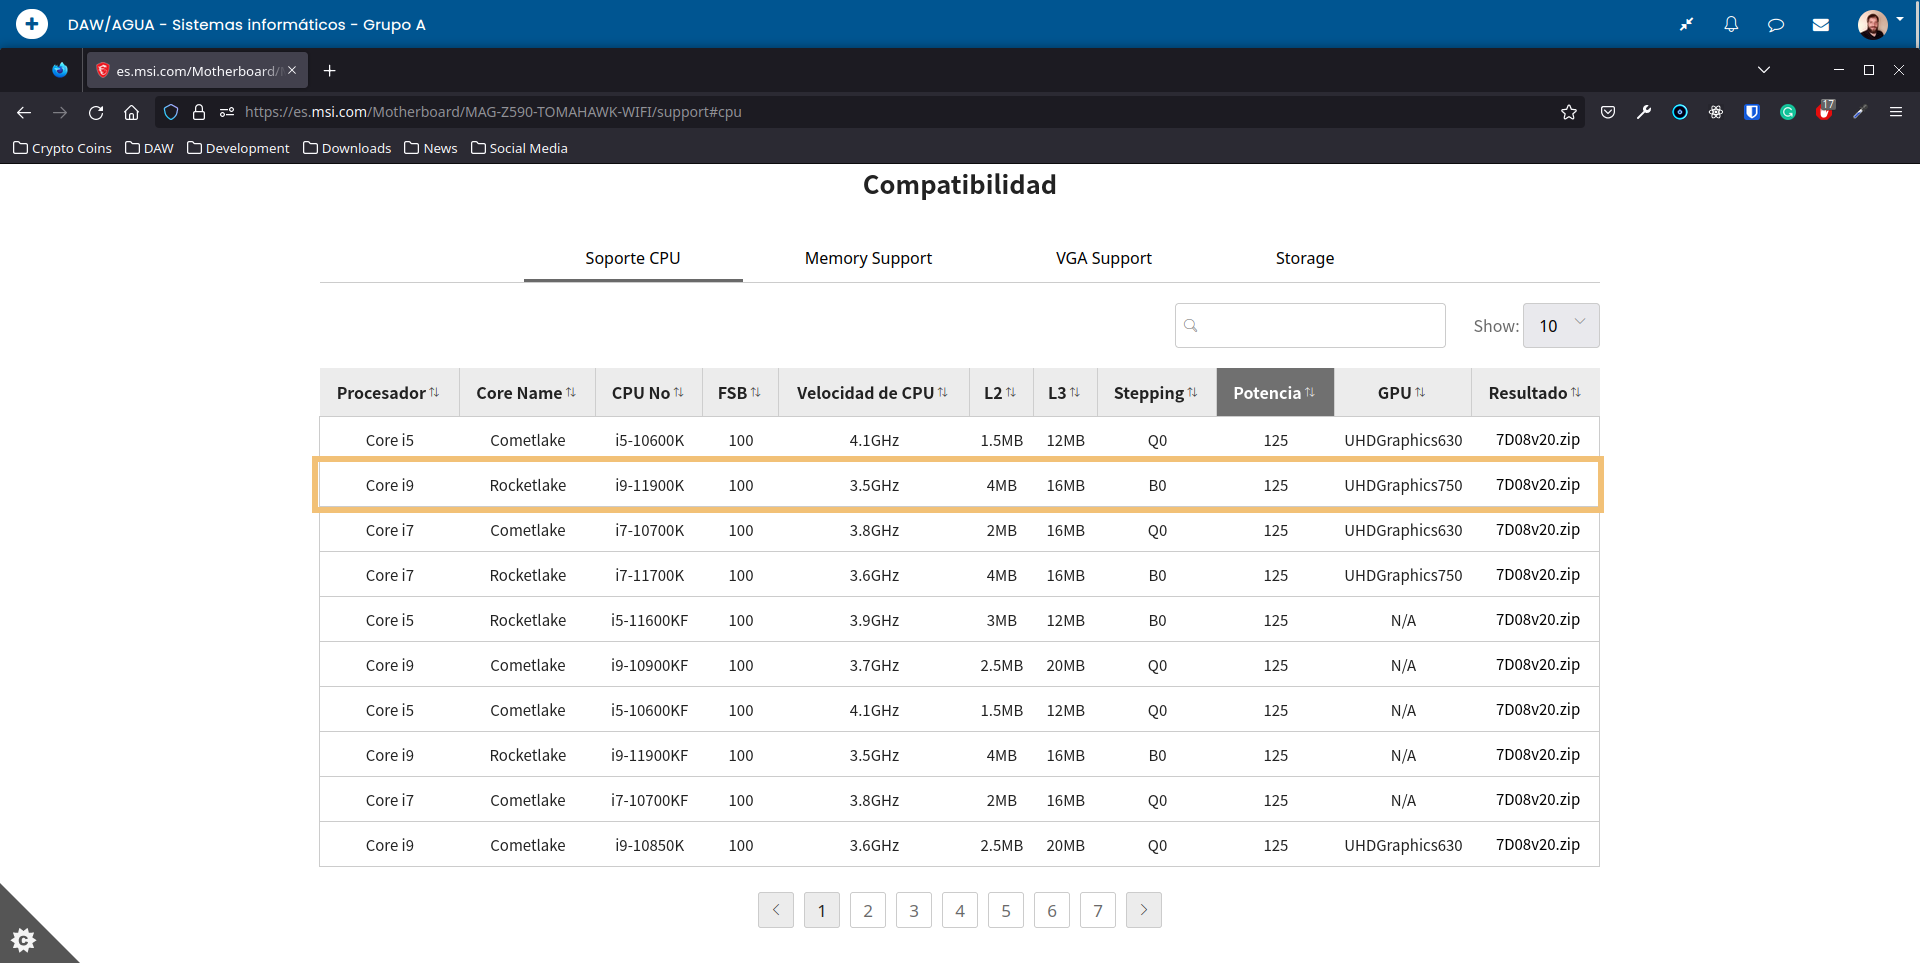
\includegraphics[scale=0.27]{cpu-potente.png}
         \caption{Página web de compatibilidad de MSI}
     \end{figure}
\end{enumerate}

% Bibliography

\newpage
\bibliography{citas}
\bibliographystyle{unsrt}

\end{document}